% Provenance (never printed): cycle 4 SVT/physique, "La planete Terre,
% l'environnement": the movements of the atmosphere, weather and its
% forecast; see sources/book1/PROVENANCE.md. Book 1, grade 8, chapter 3.
% Vocabulary guard: owns air mass, front (warm, cold), depression (homograph:
% phrase-level linking only), anticyclone, isobar, weather forecast. The
% rotation of the winds around lows and highs is told (deflection, recalled
% from ch. g8.2); the occluded front is named in prose only; numerical models
% are told, not taught.
\chapter{Massas de ar, frentes e mapas do tempo}\label{ch:g8:fronts-and-weather-maps}

A manhã está clara e sem vento. Perto do meio-dia, finos riscos brancos
aparecem bem alto no céu, e se espalham devagar num véu pálido que apaga
o Sol. À tarde, as \omterm{def:g4:clouds-rain-snow:cloud}{nuvens} ficam mais grossas e mais baixas; à noitinha,
cai uma \omterm{def:g4:clouds-rain-snow:precipitation}{chuva} contínua. Durante a noite, o ar fica quente e úmido, e
depois uma linha escura de \omterm{def:g4:clouds-rain-snow:cloud}{nuvens} traz uma pancada curta de \omterm{def:g4:clouds-rain-snow:precipitation}{chuva} forte e
uma rajada de vento. A manhã seguinte é limpa, fresca e com vento. Em dois
dias, uma \emph{\omterm{def:g8:fronts-and-weather-maps:depression}{depressão}} passou sobre a cidade, com as suas duas \omterm{def:g8:fronts-and-weather-maps:front}{frentes}.
% ledger: ucar:warm-front, ucar:cold-front

\begin{omfigure}
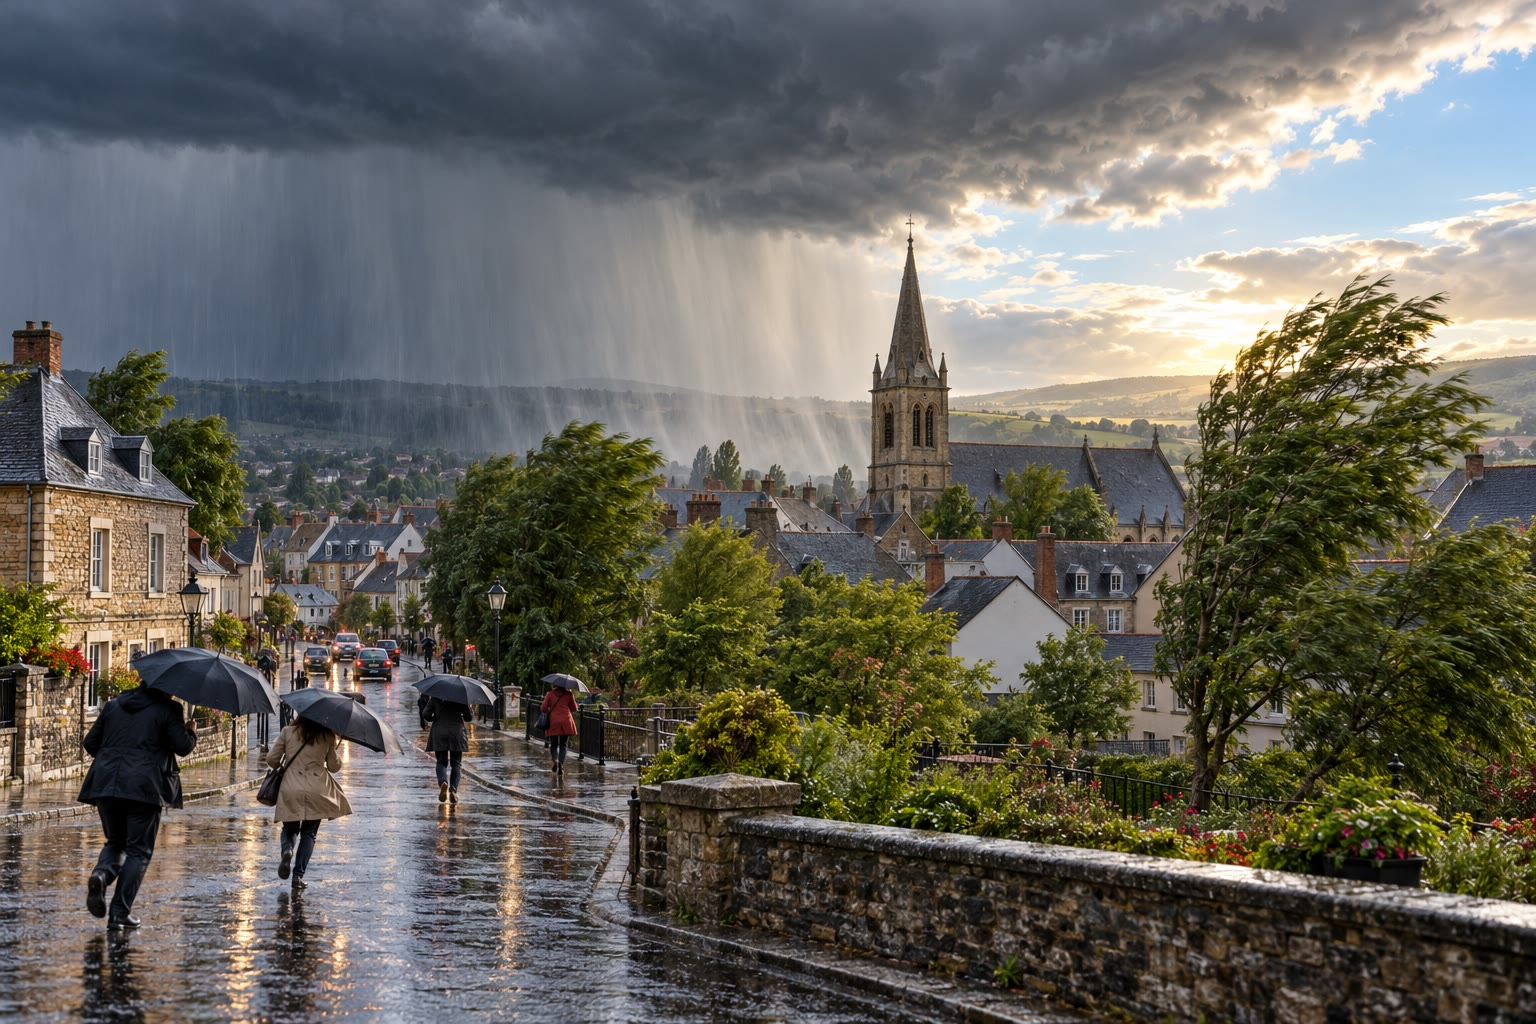
\includegraphics[width=0.6\linewidth]{images/book1/ai/g8-rain-arriving.jpg}

{\small Uma cortina de \omterm{def:g4:clouds-rain-snow:precipitation}{chuva} chega sobre uma cidade embaixo de uma base de
\omterm{def:g4:clouds-rain-snow:cloud}{nuvens} escura, enquanto o céu ainda está limpo atrás da igreja
(ilustração de uma cena genérica feita por IA).}
\label{fig:g8:fronts-and-weather-maps:rain}
\end{omfigure}

Os meteorologistas viram isso chegar dias antes. Este capítulo mostra
como: o ar do nosso céu vem em grandes massas, as massas se encontram ao
longo de \omterm{def:g8:fronts-and-weather-maps:front}{frentes}, e os \omterm{def:g2:drawing-to-map:map}{mapas} da pressão mostram para onde elas vão.

\begin{recall}
O ar faz pressão sobre tudo o que ele toca; um barômetro mede essa
pressão em hectopascais (os livros de física), e no \omterm{def:g4:world-physical-map:altitude}{nível do mar} ela é de
cerca de \qty{1013}{hPa} (\cref{ch:g8:the-atmosphere}). As \omterm{def:g4:clouds-rain-snow:cloud}{nuvens} se
formam quando o ar úmido sobe e esfria (\cref{ch:g4:clouds-rain-snow}).
No chão, o vento sopra da alta pressão para a baixa pressão, e a rotação
da Terra o desvia: para a direita no \omterm{def:g3:continents-and-oceans:equator}{hemisfério norte}. Entre cerca de
\ang{30} e \ang{60}, os \omterm{def:g8:winds-global-circulation:global-winds}{ventos de oeste} trazem uma \omterm{def:g5:natural-hazards:storm}{tempestade} atrás da
outra (\cref{ch:g8:winds-global-circulation}).
\end{recall}

\section{As massas de ar}

O ar que fica dias em cima do mesmo lugar ganha o caráter da superfície
embaixo dele. Sobre um \omterm{def:g2:water-on-earth:ocean}{oceano} quente, ele fica quente e úmido; sobre uma
terra gelada, frio e seco. Quando ele vai embora, leva esse caráter
consigo, às vezes por milhares de quilômetros.
% ledger: noaa:air-mass

\begin{definition}[Massa de ar]\label{def:g8:fronts-and-weather-maps:air-mass}
Uma \emph{massa de ar}\index{massa de ar} é um volume de ar muito grande
no qual a temperatura e a umidade são quase as mesmas em todo lugar a uma
dada \omterm{def:g4:world-physical-map:altitude}{altitude}. Ela as recebe da região onde se formou, a sua
\emph{região de origem}.
\end{definition}
% ledger: noaa:air-mass

Os meteorologistas dão a uma \omterm{def:g8:fronts-and-weather-maps:air-mass}{massa de ar} um nome de duas letras. A
primeira diz onde ela se formou: \emph{c} (continental) sobre a terra,
então ela é seca; \emph{m} (marítima) sobre um \omterm{def:g2:water-on-earth:ocean}{oceano}, então ela é úmida.
A segunda diz quão fria ela é: \emph{A} (ártica) sobre as regiões
polares, \emph{P} (polar) sobre as \omterm{def:g6:latitude-longitude:latitude}{latitudes} altas, \emph{T} (tropical)
sobre as \omterm{def:g6:latitude-longitude:latitude}{latitudes} baixas. O ar de um \omterm{def:g5:weather-and-climate:desert}{deserto} quente é cT, quente e seco;
o ar do Ártico é cA, muito frio e seco.
% ledger: noaa:air-mass

\begin{omfigure}
\begin{tikzpicture}
\begin{axis}[ommap, width=12.6cm, xmin=-100, xmax=60, ymin=10, ymax=85,
  xtick={-90,-60,...,60}, ytick={20,40,60,80},
  xticklabels={$90^\circ$O,$60^\circ$O,$30^\circ$O,$0^\circ$,$30^\circ$L,$60^\circ$L},
  yticklabels={$20^\circ$N,$40^\circ$N,$60^\circ$N,$80^\circ$N},
  tick label style={font=\scriptsize}]
  \addplot[fill=omLithAlluv, draw=black!45, line width=0.2pt] table {figdata/out/shared-geo-land.dat};
  \tikzset{src/.style={line width=0.9pt, fill opacity=0.35, text opacity=1, font=\scriptsize, align=center}}
  \draw[src, draw=omCold, fill=omCold!35] (axis cs:-30,79) ellipse [x radius=26, y radius=4.5];
  \node[font=\scriptsize, align=center, fill=white, inner sep=1pt] at (axis cs:-30,79) {\textbf{cA}: muito fria, seca};
  \draw[src, draw=omCold, fill=omCold!25] (axis cs:-35,55) ellipse [x radius=14, y radius=6];
  \node[font=\scriptsize, align=center, fill=white, inner sep=1pt] at (axis cs:-35,55) {\textbf{mP}: fria,\\ úmida};
  \draw[src, draw=omCold, fill=omCold!25] (axis cs:-84,60) ellipse [x radius=12, y radius=7];
  \node[font=\scriptsize, align=center, fill=white, inner sep=1pt] at (axis cs:-84,60) {\textbf{cP}: fria,\\ seca};
  \draw[src, draw=omCold, fill=omCold!25] (axis cs:45,62) ellipse [x radius=14, y radius=7];
  \node[font=\scriptsize, align=center, fill=white, inner sep=1pt] at (axis cs:45,62) {\textbf{cP}: fria,\\ seca};
  \draw[src, draw=omWarm, fill=omWarm!25] (axis cs:-45,28) ellipse [x radius=16, y radius=6];
  \node[font=\scriptsize, align=center, fill=white, inner sep=1pt] at (axis cs:-45,28) {\textbf{mT}: quente,\\ úmida};
  \draw[src, draw=omWarm, fill=omWarm!25] (axis cs:10,24) ellipse [x radius=15, y radius=6];
  \node[font=\scriptsize, align=center, fill=white, inner sep=1pt] at (axis cs:10,24) {\textbf{cT}: muito quente,\\ seca};
\end{axis}
\end{tikzpicture}

{\small Regiões de origem típicas das \omterm{def:g8:fronts-and-weather-maps:air-mass}{massas de ar} em volta do Atlântico
Norte (esquema): sobre o Ártico, os \omterm{def:g3:continents-and-oceans:continent}{continentes} frios, o \omterm{def:g2:water-on-earth:ocean}{oceano} do norte,
o \omterm{def:g2:water-on-earth:ocean}{oceano} subtropical e o Saara. Azul: \omterm{def:g8:fronts-and-weather-maps:air-mass}{massas de ar} frias; vermelho:
massas quentes.}
% ledger: noaa:air-mass, data:ne-land (schematic regions)
\label{fig:g8:fronts-and-weather-maps:sources}
\end{omfigure}

\section{As frentes}

Quando uma \omterm{def:g8:fronts-and-weather-maps:air-mass}{massa de ar} se desloca, ela encontra outra. As duas não se
misturam com facilidade: elas ficam separadas, com uma fronteira estreita
entre elas, onde o \omterm{def:g1:watching-the-weather:weather}{tempo} muda.
% ledger: mo:fronts, ucar:cold-front

\begin{definition}[Frente]\label{def:g8:fronts-and-weather-maps:front}
Uma \emph{frente}\index{frente} é a fronteira, no chão, entre duas \omterm{def:g8:fronts-and-weather-maps:air-mass}{massas
de ar} de temperatura e de umidade diferentes. Numa \emph{frente
fria}\index{frente fria}, o ar frio avança sobre o ar mais quente e toma o
seu lugar; numa \emph{frente quente}\index{frente quente}, o ar quente
avança sobre o ar mais frio e toma o seu lugar.
\end{definition}
% ledger: mo:fronts, ucar:cold-front, ucar:warm-front

O ar frio é mais denso que o ar quente. Numa \omterm{def:g8:fronts-and-weather-maps:front}{frente fria}, o ar frio
desliza por baixo do ar quente como uma cunha e o levanta bruscamente. O
ar quente e úmido sobe depressa e forma \omterm{def:g4:clouds-rain-snow:cloud}{nuvens} altíssimas, \omterm{def:g4:clouds-rain-snow:cloud-families}{cúmulos} e
\omterm{def:g4:clouds-rain-snow:cloud-families}{cumulonimbos}: a \omterm{def:g8:fronts-and-weather-maps:front}{frente} traz pancadas de \omterm{def:g4:clouds-rain-snow:precipitation}{chuva} forte, às vezes \omterm{def:g4:clouds-rain-snow:precipitation}{granizo} e
trovões, rajadas de vento e uma queda repentina da temperatura. Depois que
ela passa, a \omterm{def:g4:clouds-rain-snow:precipitation}{chuva} para e o céu abre. Uma \omterm{def:g8:fronts-and-weather-maps:front}{frente fria} se desloca depressa,
até duas vezes mais rápido que uma \omterm{def:g8:fronts-and-weather-maps:front}{frente quente}.
% ledger: ucar:cold-front

\begin{omfigure}
\begin{tikzpicture}[font=\footnotesize, >={Stealth[length=2.2mm]}, yscale=0.7, xscale=0.95]
  % ground
  \draw[line width=0.8pt] (0,0) -- (15,0);
  % cold wedge, nose at x = 8.2
  \fill[omCold!18] (0,0) -- (0,3.4) .. controls (4.5,3.2) and (7.2,2.4) .. (7.9,0.8)
    .. controls (8.1,0.35) and (8.2,0.12) .. (8.25,0) -- cycle;
  \draw[omCold, line width=1pt] (0,3.4) .. controls (4.5,3.2) and (7.2,2.4) .. (7.9,0.8)
    .. controls (8.1,0.35) and (8.2,0.12) .. (8.25,0);
  \node[omCold, align=center] at (3.2,1.4) {\textbf{ar frio}\\(denso)};
  \node[omWarm, align=center] at (12.6,1.4) {\textbf{ar quente e úmido}};
  % cold air pushes
  \draw[->, omCold, line width=1.2pt] (4.6,0.5) -- (7.0,0.5);
  % warm air lifted
  \draw[->, omWarm, line width=1.2pt] (11.2,0.45) .. controls (9.4,0.6) and (8.6,1.4) .. (8.5,3.0);
  % cumulonimbus
  \fill[black!12] (7.3,2.6) .. controls (7.0,3.4) and (7.4,4.2) .. (7.9,4.5)
    .. controls (7.6,5.0) and (8.6,5.2) .. (9.4,5.1) -- (11.0,5.15)
    .. controls (10.6,4.9) and (10.2,4.8) .. (10.0,4.6)
    .. controls (10.4,4.0) and (10.2,3.0) .. (9.8,2.5) -- cycle;
  \draw[black!45] (7.3,2.6) .. controls (7.0,3.4) and (7.4,4.2) .. (7.9,4.5)
    .. controls (7.6,5.0) and (8.6,5.2) .. (9.4,5.1) -- (11.0,5.15)
    .. controls (10.6,4.9) and (10.2,4.8) .. (10.0,4.6)
    .. controls (10.4,4.0) and (10.2,3.0) .. (9.8,2.5) -- cycle;
  \node at (9.0,3.8) {cumulonimbo};
  \foreach \x in {7.7,8.0,...,9.6} \draw[omCold!70, line width=0.5pt] (\x,2.45) -- (\x-0.25,0.15);
  \node[anchor=west, align=left] at (9.8,1.95) {chuva forte,\\rajadas};
  % motion
  \draw[->, line width=1.3pt] (5.7,4.3) -- (7.2,4.3);
  \node[anchor=east] at (5.6,4.3) {a frente avança};
  \node[anchor=north] at (8.25,-0.1) {frente no chão};
  \node[anchor=north west, align=left] at (0.1,-0.1) {atrás: mais fresco, o céu abre};
  \node[anchor=north east, align=right] at (15,-0.1) {à frente: quente, úmido};
\end{tikzpicture}

{\small Uma \omterm{def:g8:fronts-and-weather-maps:front}{frente fria} vista de lado (\omterm{def:g4:world-physical-map:altitude}{altitudes} muito exageradas). O ar
frio avança por baixo do ar quente como uma cunha; o ar quente é levantado
de maneira íngreme e forma \omterm{def:g4:clouds-rain-snow:cloud}{nuvens} altíssimas.}
% ledger: ucar:cold-front
\label{fig:g8:fronts-and-weather-maps:cold}
\end{omfigure}

Numa \omterm{def:g8:fronts-and-weather-maps:front}{frente quente}, o ar quente e leve não consegue empurrar o ar frio
para longe do chão: ele sobe devagar por cima dele, numa rampa longa e
suave. As suas \omterm{def:g4:clouds-rain-snow:cloud}{nuvens} aparecem, então, bem à frente da \omterm{def:g8:fronts-and-weather-maps:front}{frente}, lá no alto
do céu: primeiro finos riscos de \omterm{def:g4:clouds-rain-snow:cloud-families}{cirros}, depois um véu de cirrostratos, e
depois altostratos cinzentos. À medida que a \omterm{def:g8:fronts-and-weather-maps:front}{frente} se aproxima, as \omterm{def:g4:clouds-rain-snow:cloud}{nuvens}
ficam mais baixas e mais grossas, e começa uma \omterm{def:g4:clouds-rain-snow:precipitation}{chuva} longa e contínua.
Depois que ela passa, o ar fica mais quente e mais úmido.
% ledger: ucar:warm-front, bom:isobars (warm front: steady rain, grey skies)

\begin{omfigure}
\begin{tikzpicture}[font=\footnotesize, >={Stealth[length=2.2mm]}]
  \draw[line width=0.8pt] (0,0) -- (15,0);
  % cold air ahead (right), warm air climbing a gentle slope from the front at x = 2.2
  \fill[omCold!18] (2.2,0) .. controls (6,0.9) and (10,2.2) .. (15,3.4) -- (15,0) -- cycle;
  \draw[omCold, line width=1pt] (2.2,0) .. controls (6,0.9) and (10,2.2) .. (15,3.4);
  \node[omCold, align=center] at (11.8,0.75) {\textbf{ar frio}};
  \node[omWarm, align=center] at (1.4,1.6) {\textbf{ar quente}\\\textbf{e úmido}};
  \draw[->, omWarm, line width=1.2pt] (1.0,0.45) .. controls (4.5,0.9) and (8.5,2.4) .. (12.4,3.4);
  % clouds: nimbostratus near the front, altostratus, cirrostratus, cirrus far ahead
  \fill[black!18] (2.4,0.7) .. controls (3.2,1.8) and (5.5,2.3) .. (6.6,2.4) -- (6.4,1.25) .. controls (5,1.0) and (3.8,0.7) .. cycle;
  \node at (5.4,1.62) {nimbostratos};
  \foreach \x in {3.0,3.3,...,5.7} \draw[omCold!70, line width=0.5pt] (\x,0.95) -- (\x-0.2,0.25);
  \fill[black!10, rounded corners=4pt] (6.4,2.65) rectangle (10.0,3.25);
  \node at (8.2,2.95) {altostratos};
  \fill[black!6, rounded corners=4pt] (9.6,3.75) rectangle (12.6,4.15);
  \node at (11.1,3.95) {cirrostratos};
  \foreach \x in {12.6,13.2,13.8} \draw[black!35, line width=0.6pt] (\x,4.55) .. controls (\x+0.2,4.75) and (\x+0.4,4.6) .. (\x+0.55,4.85);
  \node[anchor=south] at (13.4,4.9) {cirros};
  \draw[->, line width=1.3pt] (2.6,4.3) -- (4.1,4.3);
  \node[anchor=east] at (2.5,4.3) {a frente avança};
  \node[anchor=north] at (2.2,-0.1) {frente no chão};
  \node[anchor=north east] at (15,-0.1) {bem à frente: as primeiras nuvens altas};
\end{tikzpicture}

{\small Uma \omterm{def:g8:fronts-and-weather-maps:front}{frente quente} vista de lado (\omterm{def:g4:world-physical-map:altitude}{altitudes} muito exageradas). O ar
quente sobe devagar por cima do ar frio; as suas \omterm{def:g4:clouds-rain-snow:cloud}{nuvens} ficam mais baixas
e mais grossas à medida que a \omterm{def:g8:fronts-and-weather-maps:front}{frente} se aproxima, e a \omterm{def:g4:clouds-rain-snow:precipitation}{chuva} é longa e
contínua.}
% ledger: ucar:warm-front
\label{fig:g8:fronts-and-weather-maps:warm}
\end{omfigure}

Num \omterm{def:g2:drawing-to-map:map}{mapa} do \omterm{def:g1:watching-the-weather:weather}{tempo}, uma \omterm{def:g8:fronts-and-weather-maps:front}{frente fria} é desenhada como uma linha azul com
triângulos, e uma \omterm{def:g8:fronts-and-weather-maps:front}{frente quente} como uma linha vermelha com
semicírculos. Os símbolos ficam do lado para onde a \omterm{def:g8:fronts-and-weather-maps:front}{frente} se desloca.
Quando uma \omterm{def:g8:fronts-and-weather-maps:front}{frente fria} rápida alcança uma \omterm{def:g8:fronts-and-weather-maps:front}{frente quente}, as duas se juntam
numa \emph{\omterm{def:g8:fronts-and-weather-maps:front}{frente} oclusa}, desenhada em roxo com os dois símbolos.
% ledger: mo:fronts, ucar:cold-front

\section{Depressões e anticiclones}

As \omterm{def:g8:fronts-and-weather-maps:front}{frentes} nascem nos grandes redemoinhos de ar que atravessam as
\omterm{def:g6:latitude-longitude:latitude}{latitudes} médias. Onde o ar sobe, a pressão no chão é mais baixa que em
toda a volta; onde ele desce, a pressão é mais alta.
% ledger: bom:highs-lows

\begin{definition}[Depressão e anticiclone]\label{def:g8:fronts-and-weather-maps:depression}
Uma \emph{depressão}\index{depressao (meteorologia)@depressão (meteorologia)}, ou baixa, é uma região onde
a pressão no \omterm{def:g4:world-physical-map:altitude}{nível do mar} é mais baixa que em toda a sua volta. Um
\emph{anticiclone}\index{anticiclone}, ou alta, é uma região onde ela é
mais alta que em toda a sua volta.
\end{definition}
% ledger: bom:isobars, bom:highs-lows
\phantomsection\label{def:g8:fronts-and-weather-maps:anticyclone}

O vento sopra da alta para a baixa, mas a rotação da Terra o desvia, então
ele acaba soprando quase em volta dos centros. No \omterm{def:g3:continents-and-oceans:equator}{hemisfério norte}, ele
gira no sentido anti-horário em volta de uma \omterm{def:g8:fronts-and-weather-maps:depression}{depressão} e no sentido
horário em volta de um \omterm{def:g8:fronts-and-weather-maps:depression}{anticiclone}; no \omterm{def:g3:continents-and-oceans:equator}{hemisfério sul}, é o contrário.
Numa \omterm{def:g8:fronts-and-weather-maps:depression}{depressão}, o ar entra perto do chão, sobe, esfria e forma \omterm{def:g4:clouds-rain-snow:cloud}{nuvens}: as
depressões trazem \omterm{def:g4:clouds-rain-snow:cloud}{nuvens}, \omterm{def:g4:clouds-rain-snow:precipitation}{chuva} e vento, e as suas \omterm{def:g8:fronts-and-weather-maps:front}{frentes}. Num
\omterm{def:g8:fronts-and-weather-maps:depression}{anticiclone}, o ar desce e esquenta ao descer: os \omterm{def:g8:fronts-and-weather-maps:depression}{anticiclones} trazem
\omterm{def:g1:watching-the-weather:weather}{tempo} seco e firme, com ventos fracos. Um \omterm{def:g8:fronts-and-weather-maps:depression}{anticiclone} típico tem uma
pressão de cerca de \qty{1020}{hPa} ou mais no seu centro; uma \omterm{def:g8:fronts-and-weather-maps:depression}{depressão}
profunda cai abaixo de \qty{980}{hPa}.
% ledger: bom:highs-lows, bom:isobars, mo:global-circ

\begin{omfigure}
\begin{minipage}[c]{0.36\linewidth}\centering
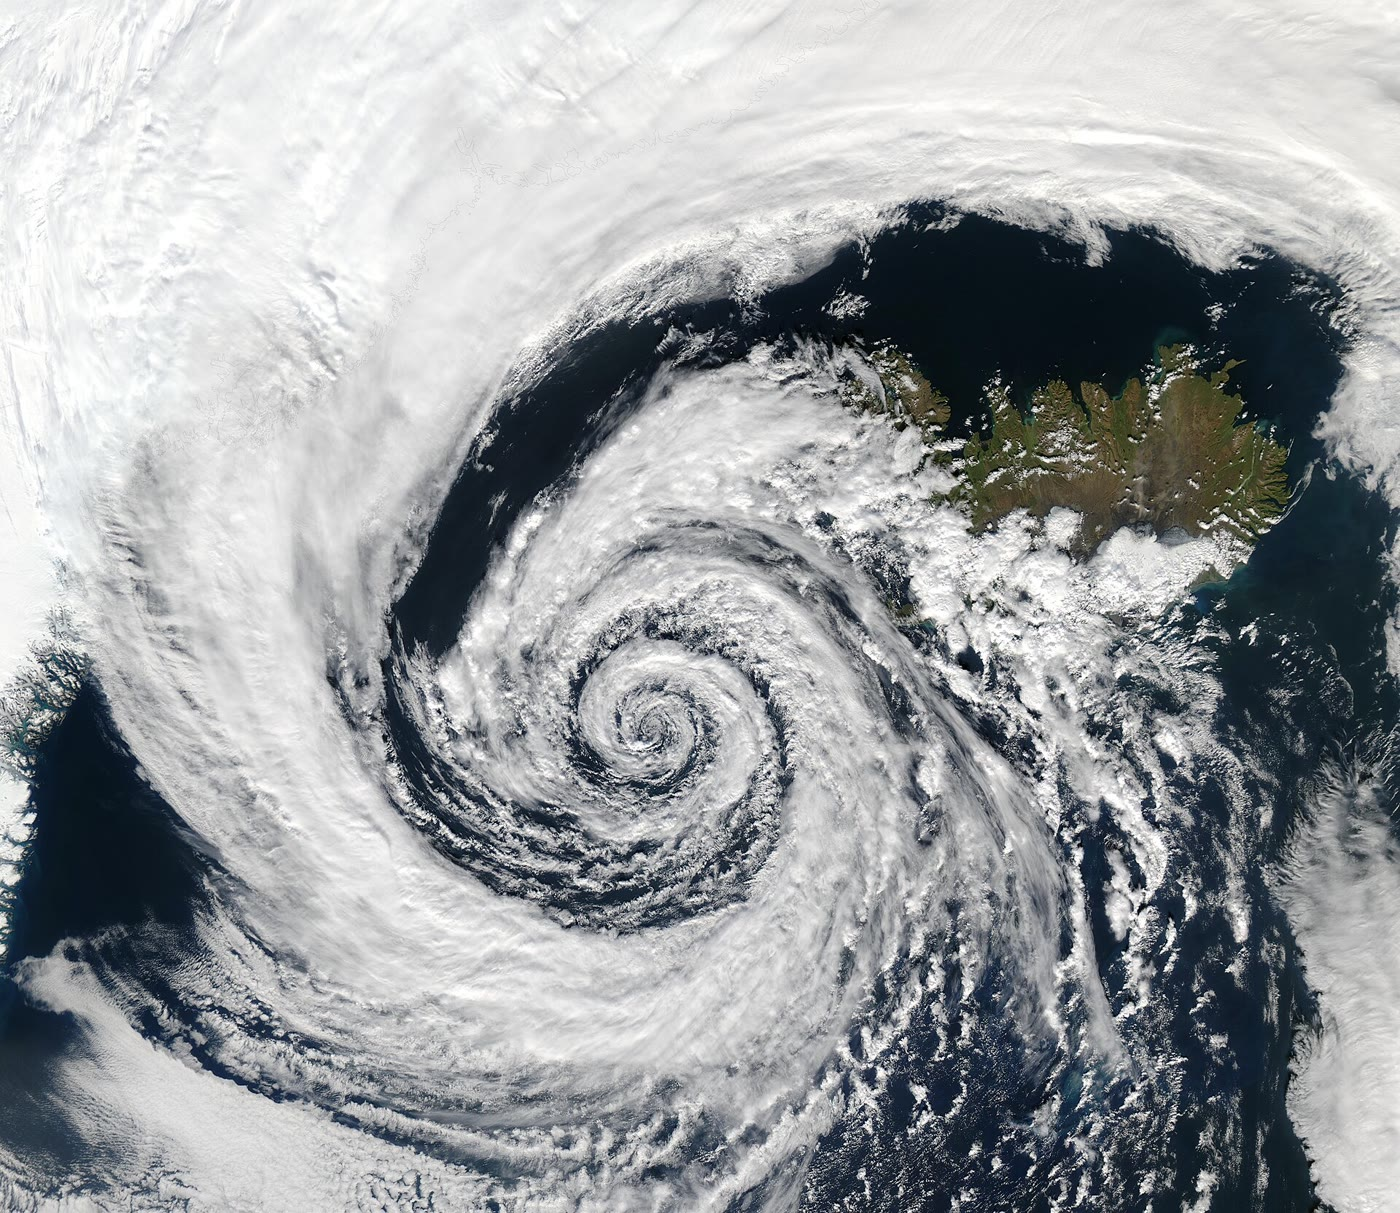
\includegraphics[width=\linewidth]{images/book1/g8-iceland-low.jpg}
\end{minipage}\hfill
\begin{minipage}[c]{0.6\linewidth}\raggedright
{\small Uma \omterm{def:g8:fronts-and-weather-maps:depression}{depressão} a sudoeste da Islândia (a ilha no alto, à direita)
vista pelo satélite Aqua da NASA em 4~de~setembro~de~2003. As suas \omterm{def:g4:clouds-rain-snow:cloud}{nuvens}
espiralam em direção ao centro, girando no sentido anti-horário como em
toda \omterm{def:g8:fronts-and-weather-maps:depression}{depressão} do \omterm{def:g3:continents-and-oceans:equator}{hemisfério norte}. NASA/GSFC, MODIS Rapid Response Team,
Jacques Descloitres (domínio público, via Wikimedia Commons).}
\end{minipage}
% ledger: commons:iceland-low, bom:highs-lows
\label{fig:g8:fronts-and-weather-maps:iceland}
\end{omfigure}

\section{As isóbaras e os mapas do tempo}

Para ver as depressões e os \omterm{def:g8:fronts-and-weather-maps:depression}{anticiclones}, os meteorologistas desenham
\omterm{def:g2:drawing-to-map:map}{mapas} da pressão. Cada estação mede a sua pressão e a reduz ao \omterm{def:g4:world-physical-map:altitude}{nível do
mar}, para que uma estação numa \omterm{def:g1:landscapes-around-us:landform}{montanha} possa ser comparada com uma no
\omterm{def:g1:landscapes-around-us:water}{litoral}. Depois, traçam-se linhas por todos os lugares onde a pressão é a
mesma.
% ledger: bom:isobars

\begin{definition}[Isóbara]\label{def:g8:fronts-and-weather-maps:isobar}
Uma \emph{isóbara}\index{isobara@isóbara} é uma linha num \omterm{def:g2:drawing-to-map:map}{mapa} que liga os
lugares onde a pressão no \omterm{def:g4:world-physical-map:altitude}{nível do mar} é a mesma. As isóbaras são
indicadas em hectopascais e muitas vezes traçadas de \qty{4}{hPa} em
\qty{4}{hPa}.
\end{definition}
% ledger: bom:isobars (the 4 hPa step is the one of this book's maps)

Em volta de uma \omterm{def:g8:fronts-and-weather-maps:depression}{depressão}, as \omterm{def:g8:fronts-and-weather-maps:isobar}{isóbaras} formam circuitos fechados, com a
pressão mais baixa no centro, marcado com a letra L, o símbolo
internacional da baixa pressão; em volta de um \omterm{def:g8:fronts-and-weather-maps:depression}{anticiclone}, elas formam
circuitos com a pressão mais alta no centro, marcado com a letra H, o da
alta pressão. Onde as \omterm{def:g8:fronts-and-weather-maps:isobar}{isóbaras} estão próximas umas das outras, a pressão
muda depressa de um lugar para o seguinte, e o vento é forte; onde elas
estão afastadas, o vento é fraco.
% ledger: bom:isobars

\begin{omfigure}
\begin{tikzpicture}
\begin{axis}[width=14cm, axis equal image, xmin=0, xmax=2400, ymin=0, ymax=1600,
  hide axis, clip=true, axis background/.style={fill=white}]
  \addplot[isobar] table {figdata/out/grade-8-weather_map-isobars.dat};
  \addplot[warm front] table {figdata/out/grade-8-weather_map-warm.dat};
  \addplot[cold front] table {figdata/out/grade-8-weather_map-cold.dat};
  \addplot[quiver={u=\thisrow{u}, v=\thisrow{v}}, -{Stealth[length=1.5mm]}, omMeth, line width=0.6pt]
    table[x=x, y=y] {figdata/out/grade-8-weather_map-winds.dat};
  \addplot[only marks, mark=none, nodes near coords, point meta=explicit symbolic,
    every node near coord/.style={anchor=center, font=\tiny, fill=white, inner sep=0.6pt}]
    table[x=x, y=y, meta=level] {figdata/out/grade-8-weather_map-labels.dat};
  \node[font=\Large\bfseries, omCold, fill=white, inner sep=1pt] at (axis cs:690,1010) {L};
  \node[font=\scriptsize, anchor=north, fill=white, inner sep=0.5pt] at (axis cs:690,968) {980};
  \node[font=\Large\bfseries, omWarm] at (axis cs:1950,520) {H};
  \node[font=\scriptsize, anchor=north] at (axis cs:1950,485) {1034};
  \addplot[only marks, mark=square*, mark size=2pt, black] table[x=x, y=y] {figdata/out/grade-8-weather_map-town.dat};
  \node[font=\footnotesize\bfseries, anchor=west, fill=white, inner sep=1pt] at (axis cs:870,380) {T};
  \fill[white] (axis cs:1930,1450) rectangle (axis cs:2290,1585);
  \draw[line width=1pt] (axis cs:1950,1480) -- (axis cs:2250,1480);
  \pgfplotsinvokeforeach{1950,2050,2150,2250}{\draw (axis cs:#1,1460) -- (axis cs:#1,1500);}
  \node[font=\scriptsize, anchor=south] at (axis cs:2100,1495) {300 km};
\end{axis}
\end{tikzpicture}

{\small Um \omterm{def:g2:drawing-to-map:map}{mapa} do \omterm{def:g1:watching-the-weather:weather}{tempo} de um dia imaginário no \omterm{def:g3:continents-and-oceans:equator}{hemisfério norte},
calculado a partir de um modelo da pressão. \omterm{def:g8:fronts-and-weather-maps:isobar}{Isóbaras} de \qty{4}{hPa} em
\qty{4}{hPa}; a \omterm{def:g8:fronts-and-weather-maps:depression}{depressão} L (\qty{980}{hPa}) traz uma \omterm{def:g8:fronts-and-weather-maps:front}{frente quente}
(vermelha) e uma \omterm{def:g8:fronts-and-weather-maps:front}{frente fria} (azul); o \omterm{def:g8:fronts-and-weather-maps:depression}{anticiclone} H (\qty{1034}{hPa})
fica a leste. Setas verdes: o vento, mais longas onde ele é mais forte.
T: a cidade do problema.}
% ledger: bom:isobars, bom:highs-lows, mo:fronts (figdata/grade-8/weather_map.py)
\label{fig:g8:fronts-and-weather-maps:map}
\end{omfigure}

\begin{method}[Ler um mapa do tempo]
\begin{enumerate}
  \item Encontre os centros: L para as depressões, H para os
        \omterm{def:g8:fronts-and-weather-maps:depression}{anticiclones}, com as suas pressões.
  \item Leia as \omterm{def:g8:fronts-and-weather-maps:isobar}{isóbaras}: os seus valores sobem em direção a H e descem
        em direção a L. \omterm{def:g8:fronts-and-weather-maps:isobar}{Isóbaras} próximas significam vento forte.
  \item Encontre a direção do vento: no \omterm{def:g3:continents-and-oceans:equator}{hemisfério norte}, ele sopra quase
        ao longo das \omterm{def:g8:fronts-and-weather-maps:isobar}{isóbaras}, com a baixa pressão à sua esquerda,
        desviado um pouco em direção à baixa.
  \item Encontre as \omterm{def:g8:fronts-and-weather-maps:front}{frentes} e o sentido em que elas se deslocam (o lado
        dos seus símbolos), e depois o ar de cada lado: o que vem a
        seguir?
\end{enumerate}
\end{method}
% ledger: bom:isobars, bom:highs-lows, mo:fronts

\begin{example}[O tempo na cidade T]
No \omterm{def:g2:drawing-to-map:map}{mapa}, T fica ao sul da \omterm{def:g8:fronts-and-weather-maps:front}{frente quente} e a leste da \omterm{def:g8:fronts-and-weather-maps:front}{frente fria}: no ar
quente entre as duas \omterm{def:g8:fronts-and-weather-maps:front}{frentes}. A \omterm{def:g8:fronts-and-weather-maps:front}{frente quente} já passou por ela. As
\omterm{def:g8:fronts-and-weather-maps:isobar}{isóbaras} vão do sudoeste para o nordeste ali, com a baixa a noroeste: o
vento sopra do sudoeste, quente e úmido. A \omterm{def:g8:fronts-and-weather-maps:front}{frente fria} vem do oeste. Os
seus triângulos apontam para o leste, em direção à cidade: em poucas
horas haverá um curto período de \omterm{def:g4:clouds-rain-snow:precipitation}{chuva} forte e rajadas, depois o vento
vai virar para oeste ou noroeste, o ar vai ficar mais fresco e o céu vai
abrir.
\end{example}
% ledger: ucar:cold-front (figdata/grade-8/weather_map.py: wind at T from 227 degrees)

Um barômetro dá o seu próprio aviso, mesmo sem \omterm{def:g2:drawing-to-map:map}{mapa}. Suponha que o \omterm{def:g2:drawing-to-map:map}{mapa}
inteiro acima se deslocasse para o leste, sem mudar, a \qty{40}{km} por
hora, e que um barômetro registrador estivesse numa estação S, a leste das
\omterm{def:g8:fronts-and-weather-maps:front}{frentes}. Em dois dias e meio, ele traçaria o registro abaixo.

\begin{omfigure}
\begin{tikzpicture}
\begin{axis}[width=0.86\linewidth, height=5.4cm, xmin=0, xmax=60, ymin=980, ymax=1040,
  xtick={0,12,...,60}, ytick={980,990,...,1040},
  xlabel={horas desde o começo do registro}, ylabel={pressão (hPa)},
  axis x line=bottom, axis y line=left, axis line style={-},
  grid=major, grid style={black!10},
  tick label style={font=\scriptsize}, label style={font=\small}, clip=false]
  \draw[omWarm!80!black, dashed] (axis cs:26.28,980) -- (axis cs:26.28,1040);
  \draw[omCold!80!black, dashed] (axis cs:38.49,980) -- (axis cs:38.49,1040);
  \node[font=\scriptsize, omWarm!80!black, anchor=south, fill=white, inner sep=1pt] at (axis cs:26.28,1032) {frente quente};
  \node[font=\scriptsize, omCold!80!black, anchor=south, fill=white, inner sep=1pt] at (axis cs:38.49,1032) {frente fria};
  \addplot[black!80, line width=1pt] table[x=hour, y=p_hPa] {figdata/out/grade-8-barogram-trace.dat};
  \node[font=\scriptsize, anchor=north west, align=left] at (axis cs:2,1028) {anticiclone:\\tempo firme};
  \node[font=\scriptsize, anchor=west] at (axis cs:39.5,986) {mínimo};
\end{axis}
\end{tikzpicture}

{\small O registro de um barômetro na estação S enquanto o \omterm{def:g2:drawing-to-map:map}{mapa} acima se
desloca para o leste a \qty{40}{km} por hora (uma situação inventada,
calculada a partir do campo de pressão do \omterm{def:g2:drawing-to-map:map}{mapa}). Linhas tracejadas: a
passagem da \omterm{def:g8:fronts-and-weather-maps:front}{frente quente} e da \omterm{def:g8:fronts-and-weather-maps:front}{frente fria} pela estação.}
% ledger: (invented region: weather situation of figdata/grade-8/weather_map.py, record from figdata/grade-8/barogram.py)
\end{omfigure}

\begin{example}[Ler o registro de um barômetro]\label{ex:g8:fronts-and-weather-maps:barogram}
Durante as 8 primeiras horas, a pressão sobe até cerca de
\qty{1031}{hPa}: o \omterm{def:g8:fronts-and-weather-maps:depression}{anticiclone} passa sobre S, com \omterm{def:g1:watching-the-weather:weather}{tempo} firme. Depois ela
cai durante 30 horas, cerca de \qty{45}{hPa}: a \omterm{def:g8:fronts-and-weather-maps:depression}{depressão} está chegando. Ela cai mais depressa algumas horas
antes da passagem da \omterm{def:g8:fronts-and-weather-maps:front}{frente quente}, mais devagar no ar quente atrás dela,
e chega ao seu mínimo, cerca de \qty{986}{hPa}, bem quando a \omterm{def:g8:fronts-and-weather-maps:front}{frente fria}
passa. Depois ela sobe: a \omterm{def:g8:fronts-and-weather-maps:depression}{depressão} está se afastando, e chega o ar mais
fresco e mais limpo de trás da \omterm{def:g8:fronts-and-weather-maps:front}{frente fria}.
% ledger: (invented region: figdata/grade-8/barogram.py), bom:highs-lows
\end{example}

\section{Como se faz uma previsão}

\begin{definition}[Previsão do tempo]\label{def:g8:fronts-and-weather-maps:forecast}
Uma \emph{previsão do tempo}\index{previsao do tempo@previsão do tempo} é uma afirmação sobre o
\omterm{def:g1:watching-the-weather:weather}{tempo} esperado num lugar nas próximas horas ou nos próximos dias,
calculada a partir de observações da atmosfera e das leis da física.
\end{definition}
% ledger: mo:how-forecasts

Uma previsão é feita em três etapas. Primeiro, os serviços meteorológicos
do mundo inteiro fazem milhões de observações todos os dias: temperatura,
\omterm{def:g4:clouds-rain-snow:precipitation}{chuva}, pressão, vento e umidade, medidos em estações no chão, no \omterm{def:g2:water-on-earth:ocean}{mar}, por
balões meteorológicos, por radar e por satélites. Depois, essas
observações alimentam modelos de computador: computadores muito potentes
calculam, passo a passo, como a atmosfera vai mudar a partir do seu
estado atual. Por fim, os meteorologistas leem os resultados, comparam-nos
com o que sabem da sua região, e redigem a previsão.
% ledger: mo:how-forecasts

\begin{history}[A primeira previsão pública]
Em 1854, um oficial da marinha, Robert FitzRoy, foi posto à frente de um
novo escritório meteorológico em Londres. Toda manhã, às 9~h, estações em
todo o \omterm{def:g1:landscapes-around-us:water}{litoral} mediam o \omterm{def:g1:watching-the-weather:weather}{tempo} e mandavam as suas leituras a Londres pelo
telégrafo, a invenção mais nova da época. Em 1859, uma \omterm{def:g5:natural-hazards:storm}{tempestade}
terrível, o vendaval do \emph{Royal Charter}, afundou muitos navios;
FitzRoy criou então um serviço de avisos de \omterm{def:g5:natural-hazards:storm}{tempestade} para os
marinheiros, que começou em fevereiro~de~1861. Em 1º~de~agosto~de~1861,
ele foi mais longe e publicou a primeira \omterm{def:g8:fronts-and-weather-maps:forecast}{previsão do tempo} pública num
jornal, o \emph{The Times}. As suas previsões olhavam um ou dois dias à
frente e eram muito gerais; elas foram o começo das previsões que lemos
hoje.
\end{history}
% ledger: mo:fitzroy

As previsões ficaram muito melhores. Nas últimas décadas, os
meteorologistas ganharam cerca de um dia a mais de boa previsão a cada dez
anos: uma previsão para daqui a quatro dias é hoje tão boa quanto era uma
previsão para o dia seguinte há trinta anos. Mas, quanto mais à frente uma
previsão olha, menos certa ela é, porque pequenos erros nas observações
de partida crescem à medida que o computador avança no tempo.
% ledger: bauer:day-per-decade, mo:accuracy

\begin{inthefield}[Observar a chegada de uma frente]
Num dia em que a previsão anuncia uma \omterm{def:g8:fronts-and-weather-maps:front}{frente}, olhe para o céu a cada
poucas horas e anote o horário, as \omterm{def:g4:clouds-rain-snow:cloud}{nuvens}, o vento e a temperatura. Antes
de uma \omterm{def:g8:fronts-and-weather-maps:front}{frente quente}, os finos riscos de \omterm{def:g4:clouds-rain-snow:cloud-families}{cirros} vêm primeiro? Quando uma
\omterm{def:g8:fronts-and-weather-maps:front}{frente fria} passa, a temperatura cai e o vento muda? Compare as suas
anotações com o \omterm{def:g2:drawing-to-map:map}{mapa} do \omterm{def:g1:watching-the-weather:weather}{tempo} do dia.
\end{inthefield}

\section{Exercícios}

\begin{exercise}[$\star$]\label{exo:g8:fronts-and-weather-maps:1}
Dê o significado de cada par de letras e diga se a \omterm{def:g8:fronts-and-weather-maps:air-mass}{massa de ar} é quente ou
fria, úmida ou seca: (a) mT; (b) cP; (c) cT; (d) mP.
\end{exercise}

\begin{exercise}[$\star$]\label{exo:g8:fronts-and-weather-maps:2}
Ligue cada sinal de um \omterm{def:g2:drawing-to-map:map}{mapa} do \omterm{def:g1:watching-the-weather:weather}{tempo} ao seu significado: uma linha azul
com triângulos; uma linha vermelha com semicírculos; uma linha que liga
lugares com a mesma pressão; a letra H; a letra L.
\end{exercise}

\begin{exercise}[$\star$]\label{exo:g8:fronts-and-weather-maps:3}
Verdadeiro ou falso? Corrija as frases falsas. (a) Os \omterm{def:g8:fronts-and-weather-maps:depression}{anticiclones} em
geral trazem \omterm{def:g1:watching-the-weather:weather}{tempo} firme. (b) As \omterm{def:g4:clouds-rain-snow:cloud}{nuvens} de uma \omterm{def:g8:fronts-and-weather-maps:front}{frente quente} chegam depois
da \omterm{def:g8:fronts-and-weather-maps:front}{frente}. (c) \omterm{def:g8:fronts-and-weather-maps:isobar}{Isóbaras} próximas significam vento fraco. (d) O ar frio é
mais denso que o ar quente.
\end{exercise}

\begin{exercise}[$\star$]\label{exo:g8:fronts-and-weather-maps:4}
No \omterm{def:g2:drawing-to-map:map}{mapa} do \omterm{def:g1:watching-the-weather:weather}{tempo} deste capítulo: (a) qual é a pressão no centro da
\omterm{def:g8:fronts-and-weather-maps:depression}{depressão}? (b) E no do \omterm{def:g8:fronts-and-weather-maps:depression}{anticiclone}? (c) Quantos hectopascais separam duas
\omterm{def:g8:fronts-and-weather-maps:isobar}{isóbaras} vizinhas? (d) Quantos hectopascais de diferença há entre a
pressão dos dois centros?
\end{exercise}

\begin{exercise}[$\star\star$]\label{exo:g8:fronts-and-weather-maps:5}
Ponha estes acontecimentos na ordem em que eles ocorrem quando uma \omterm{def:g8:fronts-and-weather-maps:front}{frente
quente} se aproxima e passa: \omterm{def:g4:clouds-rain-snow:precipitation}{chuva} contínua; finos riscos de \omterm{def:g4:clouds-rain-snow:cloud-families}{cirros}; um véu
cinzento de altostratos; ar mais quente e mais úmido; as \omterm{def:g4:clouds-rain-snow:cloud}{nuvens} ficam mais
baixas e mais grossas.
\end{exercise}

\begin{exercise}[$\star\star$]\label{exo:g8:fronts-and-weather-maps:6}
Explique por que as \omterm{def:g4:clouds-rain-snow:cloud}{nuvens} de uma \omterm{def:g8:fronts-and-weather-maps:front}{frente fria} são altíssimas, enquanto as
de uma \omterm{def:g8:fronts-and-weather-maps:front}{frente quente} se espalham em camadas. Use as palavras \emph{cunha},
\emph{íngreme}, \emph{rampa suave}.
\end{exercise}

\begin{exercise}[$\star\star$]\label{exo:g8:fronts-and-weather-maps:7}
No \omterm{def:g2:drawing-to-map:map}{mapa} do \omterm{def:g1:watching-the-weather:weather}{tempo}: (a) onde o vento é mais forte, perto de L ou perto de H?
Como você pode saber? (b) Ao norte de L, de que direção sopra o vento?
(c) E ao sul de H? (d) O vento gira no sentido horário ou anti-horário em
volta de L?
\end{exercise}

\begin{exercise}[$\star\star$]\label{exo:g8:fronts-and-weather-maps:8}
Um barômetro numa cidade marca \qty{1016}{hPa} às 6:00, \qty{1009}{hPa} às
12:00 e \qty{1003}{hPa} às 18:00. (a) Quanto a pressão cai em 12 horas?
(b) O que vem em direção à cidade, uma \omterm{def:g8:fronts-and-weather-maps:depression}{depressão} ou um \omterm{def:g8:fronts-and-weather-maps:depression}{anticiclone}? (c) Que
\omterm{def:g1:watching-the-weather:weather}{tempo} a cidade pode esperar?
\end{exercise}

\begin{exercise}[$\star\star$]\label{exo:g8:fronts-and-weather-maps:9}
Um ar que ficou uma semana sobre o Saara se desloca para o norte, sobre o
\omterm{def:g2:water-on-earth:ocean}{mar} Mediterrâneo. (a) Dê o nome dessa \omterm{def:g8:fronts-and-weather-maps:air-mass}{massa de ar} com as suas duas
letras. (b) Ela é quente ou fria, úmida ou seca, quando parte? (c) O que
poderia mudar no seu caráter enquanto ela atravessa o \omterm{def:g2:water-on-earth:ocean}{mar}?
\end{exercise}

\begin{exercise}[$\star\star$]\label{exo:g8:fronts-and-weather-maps:10}
Uma previsão para daqui a quatro dias é hoje tão boa quanto era uma
previsão para o dia seguinte há trinta anos. (a) Quantos dias de boa
previsão foram ganhos em trinta anos? (b) Quantos isso dá a cada dez
anos? (c) Se o mesmo progresso continuasse, em quantos anos uma previsão
para daqui a cinco dias seria tão boa quanto a previsão de hoje para o dia
seguinte?
\end{exercise}

\begin{exercise}[$\star\star\star$]\label{exo:g8:fronts-and-weather-maps:11}
No \omterm{def:g2:drawing-to-map:map}{mapa} do \omterm{def:g1:watching-the-weather:weather}{tempo}, use a barra de \omterm{def:g2:drawing-to-map:scale}{escala}. (a) Aproximadamente quantos
quilômetros separam o centro L do centro H? (b) Perto de L, duas \omterm{def:g8:fronts-and-weather-maps:isobar}{isóbaras}
vizinhas ficam a cerca de \qty{80}{km} uma da outra. Quantos hectopascais
a pressão muda ali em \qty{100}{km}? (c) Perto de H, duas \omterm{def:g8:fronts-and-weather-maps:isobar}{isóbaras}
vizinhas ficam a cerca de \qty{140}{km} uma da outra. Mesma pergunta.
(d) Onde o vento é mais forte? As setas do \omterm{def:g2:drawing-to-map:map}{mapa} concordam?
\end{exercise}

\begin{exercise}[$\star\star\star$]\label{exo:g8:fronts-and-weather-maps:12}
Uma \omterm{def:g8:fronts-and-weather-maps:front}{frente fria} fica a \qty{300}{km} a oeste de uma cidade e se desloca
para o leste a \qty{50}{km} por hora; uma \omterm{def:g8:fronts-and-weather-maps:front}{frente quente} fica a
\qty{200}{km} a oeste de outra cidade e se desloca com a metade dessa
velocidade. (a) Que \omterm{def:g8:fronts-and-weather-maps:front}{frente} chega primeiro à sua cidade, e quantas horas
antes? (b) Descreva o \omterm{def:g1:watching-the-weather:weather}{tempo} que cada cidade vai ver quando a sua \omterm{def:g8:fronts-and-weather-maps:front}{frente}
passar. (c) Que cidade vai estar mais quente depois que a sua \omterm{def:g8:fronts-and-weather-maps:front}{frente}
passar?
\end{exercise}

\section{Problema: O jogo vai ser cancelado por causa da chuva?}

\begin{problem}[{Problema de fim de semana --- um jogo de futebol está
marcado para as 15:00 na cidade T do mapa do tempo; a frente fria está
chegando: a sua velocidade é medida em dois mapas e prevê-se a hora em
que ela chega à cidade}]
\label{pb:g8:fronts-and-weather-maps:1}
% ledger: ucar:cold-front (figdata/grade-8/weather_map.py; the front's speed and the length of the showers are exercise data)
Às 09:00, uma jovem meteorologista olha o \omterm{def:g2:drawing-to-map:map}{mapa} do \omterm{def:g1:watching-the-weather:weather}{tempo} deste capítulo, e
depois o \omterm{def:g2:drawing-to-map:map}{mapa} abaixo: ele mostra a \omterm{def:g8:fronts-and-weather-maps:front}{frente fria} perto da cidade às 06:00 e
às 09:00, numa malha de quadrados de \qty{20}{km}.

\begin{center}
\begin{tikzpicture}
\begin{axis}[width=11cm, axis equal image, xmin=0, xmax=600, ymin=0, ymax=400,
  xtick={0,100,...,600}, ytick={0,100,...,400}, minor tick num=4,
  grid=both, minor grid style={black!10}, major grid style={black!25},
  tick label style={font=\scriptsize}, xlabel={distância para leste (km)}, ylabel={distância para norte (km)},
  label style={font=\small}]
  \addplot[cold front, densely dashed, opacity=0.55] table[x expr=\thisrow{x}-363.2, y expr=\thisrow{y}-180] {figdata/out/grade-8-weather_map-seq-06.dat};
  \addplot[cold front] table[x expr=\thisrow{x}-363.2, y expr=\thisrow{y}-180] {figdata/out/grade-8-weather_map-seq-09.dat};
  \addplot[only marks, mark=square*, mark size=2.2pt, black] table[x expr=\thisrow{x}-363.2, y expr=\thisrow{y}-180] {figdata/out/grade-8-weather_map-town.dat};
  \node[font=\footnotesize\bfseries, anchor=south west, fill=white, inner sep=1pt] at (axis cs:485,205) {T};
  \node[font=\scriptsize, fill=white, inner sep=1pt] at (axis cs:140,360) {06:00};
  \node[font=\scriptsize, fill=white, inner sep=1pt] at (axis cs:262,360) {09:00};
\end{axis}
\end{tikzpicture}
\end{center}

\noindent\textbf{Parte I --- Ler o mapa.}\par\nopagebreak
\begin{enumerate}[beginpenalty=10000]
  \item No \omterm{def:g2:drawing-to-map:map}{mapa} do \omterm{def:g1:watching-the-weather:weather}{tempo} do capítulo, a cidade está no ar quente ou no ar
        frio? Que \omterm{def:g8:fronts-and-weather-maps:front}{frente} já passou por ela?
  \item De que direção o vento sopra na cidade?
  \item Para que lado a \omterm{def:g8:fronts-and-weather-maps:front}{frente fria} se desloca? Como você pode saber
        pelos seus símbolos?
  \item Que \omterm{def:g1:watching-the-weather:weather}{tempo} a \omterm{def:g8:fronts-and-weather-maps:front}{frente fria} vai trazer quando passar?
\end{enumerate}

\noindent\textbf{Parte II --- A velocidade da frente.}\par\nopagebreak
\begin{enumerate}[resume, beginpenalty=10000]
  \item No \omterm{def:g2:drawing-to-map:map}{mapa} acima, na altura da cidade, a que distância para leste
        fica a \omterm{def:g8:fronts-and-weather-maps:front}{frente} às 06:00? E às 09:00?
  \item Quantos quilômetros a \omterm{def:g8:fronts-and-weather-maps:front}{frente} andou nessas três horas?
  \item Qual é a sua velocidade, em quilômetros por hora?
  \item Às 09:00, quantos quilômetros separam a \omterm{def:g8:fronts-and-weather-maps:front}{frente} da cidade?
\end{enumerate}

\noindent\textbf{Parte III --- A previsão.}\par\nopagebreak
\begin{enumerate}[resume, beginpenalty=10000]
  \item Se a \omterm{def:g8:fronts-and-weather-maps:front}{frente} mantiver a mesma velocidade, de quantas horas ela vai
        precisar para chegar à cidade?
  \item A que horas ela vai chegar à cidade?
  \item Suponha que as pancadas de \omterm{def:g4:clouds-rain-snow:precipitation}{chuva} forte durem cerca de uma hora
        depois da passagem da \omterm{def:g8:fronts-and-weather-maps:front}{frente}. Ainda vai estar chovendo às 15:00?
  \item A \omterm{def:g8:fronts-and-weather-maps:front}{frente} poderia desacelerar para \qty{30}{km} por hora. Quando
        ela chegaria à cidade, então? Escreva a previsão para o jogo em
        uma ou duas frases, dando os dois horários possíveis.
\end{enumerate}
\end{problem}
